\documentclass[tikz,border=10pt]{standalone}
% Only the base tikz package is used (no extra TikZ libraries needed).
\begin{document}
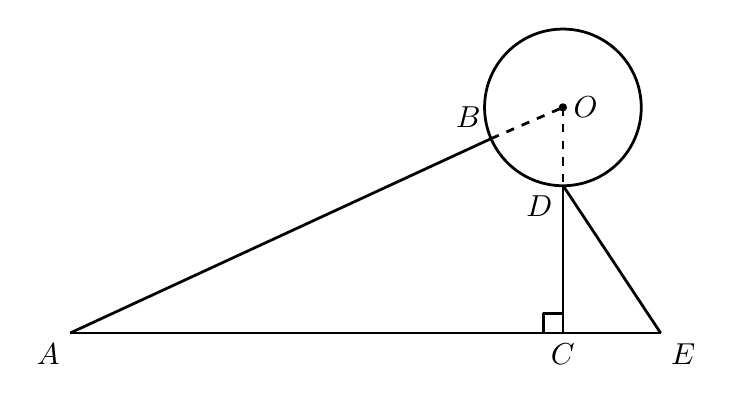
\begin{tikzpicture}[line join=round, line width=1.0pt,
    lbl/.style={font=\fontsize{10.5}{12.6}\selectfont}]
  % Named coordinates. Origin at C; units are cm (s = 0.013201 per px).
  \coordinate (A) at (-6.257,0);
  \coordinate (C) at (0,0);
  \coordinate (E) at (1.241,0);
  \coordinate (O) at (0,2.865);
  \coordinate (B) at (-0.911,2.469);
  \coordinate (D) at (0,1.875);

  % Baseline A-E (solid)
  \draw (A) -- (E);
  % Solid A-B, ends at B on the circle (A-B passes through O)
  \draw (A) -- (B);
  % Dashed continuation B-O (rest of the same line)
  \draw[dashed] (B) -- (O);
  % Dashed vertical radius O-D
  \draw[dashed] (O) -- (D);
  % Solid vertical D-C
  \draw (D) -- (C);
  % Solid D-E
  \draw (D) -- (E);
  % Full circle centred at O (radius ~75.6 px)
  \draw (O) circle[radius=0.995];

  % Right-angle mark at C (between CA and CD), from GES mark points
  \draw (0,0.251) -- (-0.251,0.251) -- (-0.251,0);

  % Filled dot at the centre O
  \fill (O) circle[radius=1.5pt];

  % Labels
  \node[below left, lbl] at (A) {$A$};
  \node[above left, lbl] at (B) {$B$};
  \node[right, lbl] at (O) {$O$};
  \node[below left, lbl] at (D) {$D$};
  \node[below, lbl] at (C) {$C$};
  \node[below right, lbl] at (E) {$E$};
\end{tikzpicture}
\end{document}